\chapter{Numerical results}
\label{chap:results}
In this chapter we present a series of convergence and preconditioning experiments. The principal aim is to check the scalability performance of the preconditioned iterative methods for the MHD problem and the two decoupling schemes proposed in Chapter \ref{chap:precond}. \RE{We have chosen to work with the Python programming language, due to its flexibility and the availability of a large collection of external libraries that this environment offers. Python is an extremely portable platform, which allows for a nearly seamless interface between multiple languages.}

\section{Software}

Due to the complex nature of the MHD problem, a number of different libraries have been used both to discretise and then to solve the resulting systems.

The finite element software that was used to discretise \eqref{eq:mhd}, \eqref{eq:bc} is {\tt FEniCS} \cite{wells2012automated}. The core libraries used within \fenics are the problem-solving interface {\tt DOLFIN} \cite{LoggWells2010a,LoggWellsEtAl2012a},  the compiler for finite element variational forms {\tt FFC} \cite{KirbyLogg2006a,LoggOlgaardEtAl2012a,OlgaardWells2010b}, the finite element  tabulator {\tt FIAT} \cite{Kirby2012a,Kirby2004a} for creating finite element function spaces, the just-in-time compiler {\tt Instant},  the code generator {\tt UFC} \cite{AlnaesLoggEtAl2009a,AlnaesLoggEtAl2012a} and  the form language {\tt UFL} \cite{AlnaesEtAl2012,Alnaes2012a}.

Along with \fenics we have used a number of stand-alone linear algebra libraries. The main one that has been used is {\tt PETSc4PY}, which is the Python interface for {\tt PETSc} \cite{petsc-web-page,petsc-user-ref}; it has been used mainly for the iterative solvers a^^^^^s well as the blockwise preconditioning setup. The following packages were used to solve the preconditioned system: {\tt HYPRE} \cite{falgout2002hypre} as a multigrid solver and the sparse direct solvers  {\tt UMFPACK} \cite{Davis:2004:CPS:992200.992205,Davis:2004:AUV:992200.992206,Davis:1999:CUM:305658.287640,davis1997unsymmetric}, {\tt PASTIX} \cite{henon2002pastix}, {\tt SuperLU} \cite{superlu_ug99,li05} and {\tt MUMPS} \cite{amestoy2000multifrontal,amestoy2001fully,amestoy2006hybrid}.

\section{Problem setup}
\label{sec:ProblemSetup}

When numerically solving a set of linear or non-linear equations the problem needs to be initialised: the mesh sequence, non-linear iteration stopping criteria and initial guess tolerance need to be defined. In this section, we will briefly cover these aspects. For simplicity, all our numerical experiments are based on lowest-order elements (i.e., $k=2$).

\paragraph{Mesh sequences} ~\\

\vspace{-5mm}


% To test the performance of the preconditioners from  Chapter \ref{chap:precond} and to validate the code produced by \fenics a sequence of meshes are required. To verify that the code  produces the correct convergence rates, we consider levels, $\ell$, of uniformly refined grids. T
In our tests, we consider sequences of uniformly refined simplicial grids (i.e., triangles in 2D and tetrahedra in 3D). The mesh level $\ell$ defines the number of edges between the nodes along a single boundary edge to be $2^{\ell}$. For example, consider the domain to be the unit square then the third level ($\ell = 3$)  generates the uniform $8\times 8$ triangular grid given in Figure \ref{fig:2Dmesh}.
\begin{figure}[h!]
  \centering
    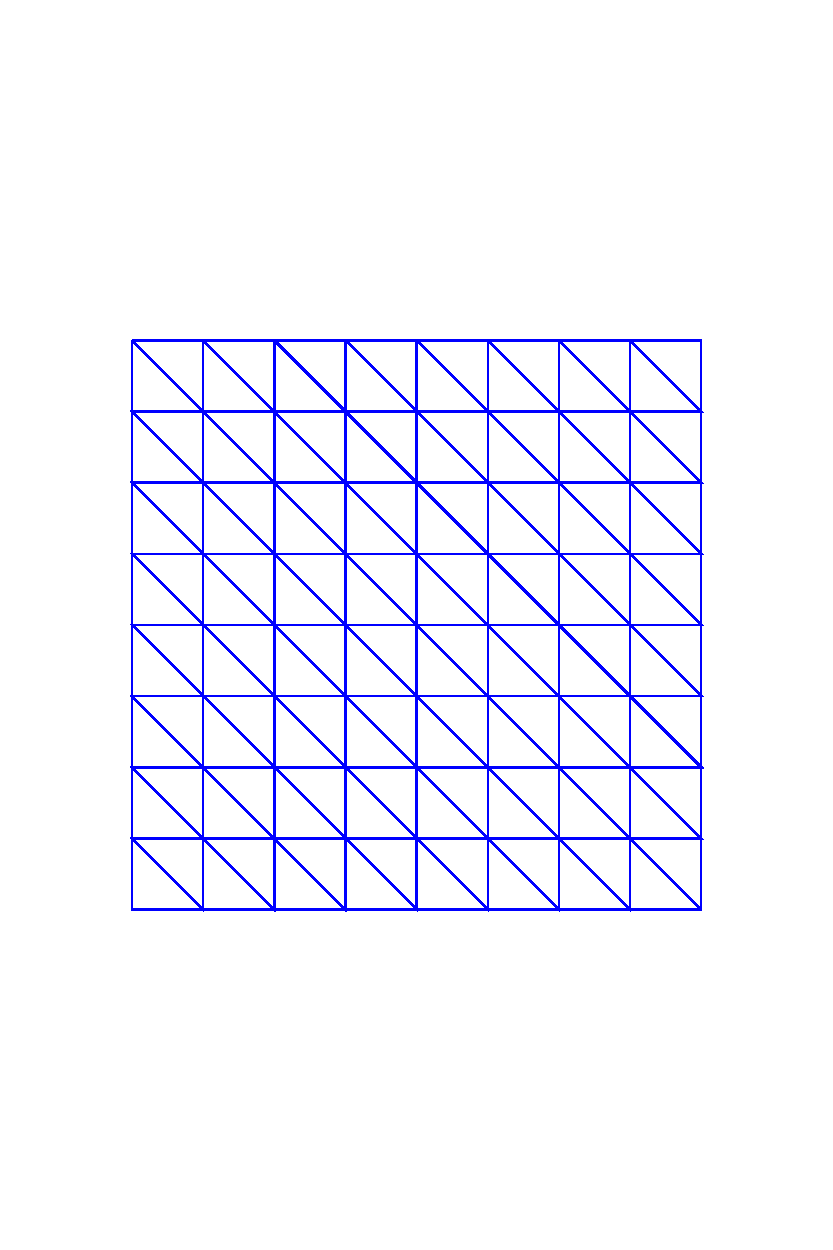
\includegraphics[scale=.5]{../Results/Figures/dolfin_plot_1}
    \caption{Level $3$ grid on unit square domain}
  \label{fig:2Dmesh}
\end{figure}
The first column of all convergence and iteration tables below will show the grid level.

\newpage

\paragraph{Stopping criteria} ~\\

\vspace{-5mm}


The incompressible Navier-Stokes equations as well as the full MHD problem are a set of non-linear equations. Section~\ref{sec:nonlinear} outlines the process in which we linearise the problem and then solve for the updates. The stopping criteria that we enforce for the Navier-Stokes and MHD problems are:
\begin{itemize}
  \item NS: $\|\delta {u} \|_2+\|\delta p \|_{2} < {tol}$,
  \item MHD: $\|\delta {u} \|_{2}+\|\delta p \|_{2}+\|\delta {b} \|_{2}+\|\delta r \|_{2} < {tol}$,
\end{itemize}
where $\|\cdot \|_2$ denotes the 2-norm of a vector. The tolerance is stated in each example table.

\RE{Note that the non-linear stopping tolerance that has been used varies from example to example. For the convergence results we set the tolerance to be stricter to make sure the convergence rates are accurate. For the preconditioning tests the tolerance is loosened slightly for ease of computation.}

% \newpage

\paragraph{Initial guess tolerance} ~\\


\vspace{-5mm}
% From the discussion in Section~\ref{sec:bcig}, we choose the Krylov tolerance for the Stokes and non-symmetric Maxwell's problems as 1e-10 and 1e-10, respectively.

To initialise the non-linear iterations, we follow Section~\ref{sec:bcig}. As discussed there, this involves iteratively solving  Stokes equations \eqref{eq:StokesInitial} and a modified Maxwell problem of the form \eqref{eq:MaxwellInitial} to a sufficient accuracy. To that end, and throughout the chapter we choose the Krylov tolerance as 1e-10 for each problem. Inhomogeneous boundary conditions are enforced in a standard fashion within the corresponding finite element spaces, by interpolation at the boundary degrees of freedom.


The notation ``Dofs'' in the tables to follow stand for the number of degrees of freedom. We usually indicate which unknowns are meant but if not then ``Dofs'' refers to the total number of degrees of freedom of the system.


\section{Numerical results: Navier-Stokes equations}
\label{sec:NS_validation}
Before considering the discretised MHD problem, we require that the Navier-Stokes subproblem perform as expected in terms of the error estimates and preconditioner scalability. To check the validity of the {\tt FEniCS} code, we introduce two problems with smooth solutions, the first in 2D and the second in 3D. \RE{As mention in Section~\ref{sec:ProblemSetup}, we only provide results lowest-order ($k=2$) Taylor-Hood elements; the discretisation in this case is stable and is sufficiently accurate for our purposes.}





\subsection{Convergence results for a 2D smooth solution}
\label{sec:2D_NS}

Consider the domain $\Omega =(0, 1)^2$. Taking the viscosity to be $\nu = 1$, we choose the source terms $\uu{f}$ and inhomogeneous Dirichlet boundary conditions on $\partial \Omega$ from the analytical solution
\begin{subequations} \nonumber
\begin{eqnarray}\nonumber
\uu{u}(x,y) &=&
\begin{pmatrix}
\sin(x)\exp(x+y)+\cos(y)\exp(x+y)\\
-\sin(y)\exp(x+y)
\end{pmatrix},\\
\nonumber
p(x,y) &=& x^3\sin(y)+\exp(x+y).
\end{eqnarray}
\end{subequations}

% Running the \fenics code produces Tables~\ref{tab:NS_2D_smooth_velocity}~and~\ref{tab:NS_2D_smooth_pressure}.
\begin{table}[h!]
\begin{center}
\begin{tabular}{cccccc}
\hline
$\ell$ &    Dofs $\uu{u}_h/p_h$ & $\|\uu{u}-\uu{u}_h\|_{L^2(\Omega)}$ & order & $\|\uu{u}-\uu{u}_h\|_{H^1(\Omega)}$ & order  \\
\hline
 3 &     578/81 &  2.2100e-04 &     - &  1.5645e-02 &     - \\
 4 &    2,178/289 &  2.7598e-05 &     3.00 &  3.9133e-03 &     2.00   \\
 5 &    8,450/1,089 &  3.4465e-06 &     3.00 &  9.7822e-04 &     2.00   \\
 6 &   33,282/4,225 &  4.3072e-07 &     3.00 &  2.4455e-04 &     2.00   \\
 7 &  132,098/16,641 &  5.3836e-08 &     3.00 &  6.1137e-05 &     2.00   \\
 8 &  526,338/66,049 &  6.7291e-09 &     3.00 &  1.5284e-05 &     2.00   \\
\hline
\end{tabular}
\caption{Convergence of the velocity field for 2D Navier-Stokes - $tol=$~1e-10}
\label{tab:NS_2D_smooth_velocity}
\end{center}
\end{table}
\begin{table}[h!]
\begin{center}
\begin{tabular}{cccccccc}
\hline
$\ell$ &    Dofs $\uu{u}_h/p_h$ &         $\|{p}-{p}_h\|_{L^2(\Omega)}$ & order \\
\hline
 3 &     578/81 &7.2758e-03 &      - \\
 4 &    2,178/289 &  1.8190e-03 &      2.00 \\
 5 &    8,450/1,089 &  4.5025e-04 &      2.01 \\
 6 &   33,282/4,225 &  1.1341e-04 &      1.99 \\
 7 &  132,098/16,641 &  2.8639e-05 &      1.99 \\
 8 &  526,338/66,049 &  7.0146e-06 &      2.03 \\


\hline
\end{tabular}
\caption{Convergence of the pressure variable for 2D Navier-Stokes - $tol=$~1e-10}
\label{tab:NS_2D_smooth_pressure}
\end{center}
\end{table}


For the lowest-order Taylor-Hood elements the expected convergence rates for the velocity field in the $L^2$- and $H^1$-norm errors are third and second order, respectively, and for the pressure the $L^2$-norm error is second order. This is in agreement with observed orders from Tables~\ref{tab:NS_2D_smooth_velocity}~and~\ref{tab:NS_2D_smooth_pressure}.
 % where we obtain third order in the $L^2$-norm errors, second order for the $H^1$-norm errors in the velocity fields and second order in the $L^2$-norm errors for the pressure.
 % This is precisely what we expect from Taylor-Hood elements.

\subsection{Convergence results for a 3D smooth solution}

The three-dimensional set up is very similar as with the 2D case. The domain is the unit cube  $\Omega =(0, 1)^3$. As before, the viscosity is $\nu = 1$, then the source term $\uu{f}$ and inhomogeneous Dirichlet boundary conditions on $\partial \Omega$ are calculated from the analytical solution
\begin{subequations} \nonumber
\begin{eqnarray}\nonumber
\uu{u}(x,y,z) &=&
\begin{pmatrix}
-\exp(x+y+z)\sin(y) + \exp(x+y+z)\sin(z)\\
\exp(x+y+z)\sin(x) - \exp(x+y+z)\sin(z)\\
-\exp(x+y+z)\sin(x) + \exp(x+y+z)\sin(y)
\end{pmatrix}, \\
\nonumber
p(x,y,z) &=&  \exp(x+y+z) + \sin(y).
\end{eqnarray}
\end{subequations}
Running the 3D code produces the results in Tables~\ref{tab:NS_3D_smooth_velocity}~and~\ref{tab:NS_3D_smooth_pressure}, which shows the computed errors and convergence rates.
\begin{table}[h!]
\begin{center}
    \begin{tabular}{cccccccc}
    \hline
    $\ell$ &    Dofs $\uu{u}_h/p_h$ & $\|\uu{u}-\uu{u}_h\|_{L^2(\Omega)}$ & order & $\|\uu{u}-\uu{u}_h\|_{H^1(\Omega)}$ & order \\
    \hline
    1 &    375/27 &  2.6211e-02 &     - &  4.5804e-01 &    -  \\
    2 &   2,187/125 &  3.2997e-03 &     2.99 &  1.1547e-01 &     1.99    \\
    3 &   14,739/729 &  4.1267e-04 &     3.00 &  2.8944e-02 &     2.00    \\
    4 &  107,811/4,913 &  5.1565e-05 &     3.00 &  7.2416e-03 &     2.00    \\
    5 &  823,875/35,937 &  6.4443e-06 &     3.00 &  1.8108e-03 &     2.00    \\
    \hline
    \end{tabular}
\caption{Convergence of the velocity field for 3D Navier-Stokes - $tol=$~1e105}
\label{tab:NS_3D_smooth_velocity}
\end{center}
\end{table}
\begin{table}[h!]
\begin{center}
    \begin{tabular}{cccccccc}
    \hline
    $\ell$ &    Dofs $\uu{u}_h/p_h$ &  $\|{p}-{p}_h\|_{L^2(\Omega)}$ & order \\
    \hline
    1 &    375/27 &  1.7725e+00 &      - \\
    2 &   2,187/125 &    2.8602e-01 &      2.63 \\
    3 &   14,739/729 &    4.0587e-02 &      2.82 \\
    4 &  107,811/4,913 &     6.4794e-03 &      2.65 \\
    5 &  823,875/35,937 &     1.2724e-03 &      2.35 \\
    \hline
    \end{tabular}
\caption{Convergence of the pressure variable for 3D Navier-Stokes - $tol=$~1e-10}
\label{tab:NS_3D_smooth_pressure}
\end{center}
\end{table}

We see that the convergence rates are the same as for the 2D test solution in the previous section for the velocity field. However, we observe that for the pressure we get a slightly higher than expected order, namely about 2.5.
% We have seen this trend for multiple different examples that have been run but never have we seen an $L^2$-norm error order lower than 2. We therefore accept this convergence behaviour.

\subsection{Preconditioning with LSC and PCD}

% Section~\ref{sec:NSprecond} outlines the two main preconditioning techniques for the Navier-Stokes equations. In order to have a scalable preconditioner for the full MHD system we need to check the performance of both LSC and PCD for the Navier-Stokes subproblem.

In this section, we check the performance of both the PCD and LSC preconditioners for the Navier-Stokes subproblem, see Sections~\ref{sec:PCD_outline}~and~\ref{sec:LSC_outline}. The problem setup is the 2D one from Section~\ref{sec:2D_NS}. We use GMRES as the Krylov subspace solver (with a convergence tolerance of 1e-5) and the application of the preconditioners will be done directly. Note that, we do not restart GMRES. The results tables show GMRES iterations averaged over all non-linear iterations.


% The tables show average number of iterations which means we calculate the average the number of GMRES iterations at each non-linear iteration.

\begin{table}[h!] \small
\begin{center}
    \begin{tabular}{cccccc}
    \hline
    $\ell$ &    Dofs &  \multicolumn{4}{ c }{Average iterations}\\
     & $\uu{u}_h/p_h$ & $\nu=10$ &  $\nu=1$ &  $\nu=0.1$&  $\nu=0.01$ \\
    \hline
     1 &      50/9 &     5 &     5 &    6 &    8 \\
     2 &     162/25 &    10 &    10 &   10 &   21 \\
     3 &     578/81 &    16 &    16 &   15 &   30 \\
     4 &    2,178/289 &    25 &    24 &   24 &   31 \\
     5 &    8,450/1,089 &    48 &    47 &   46 &   39 \\
     6 &   33,282/4,225 &   103 &    86 &   77 &   63 \\
     7 &  132,098/16,641 &   190 &   190 &  141 &  131 \\
    \hline
    \end{tabular}
\caption{Iteration table for LSC preconditioner  for 2D example for various values of $\nu$ and $tol=$~1e-5}
\label{tab:LSC_2D}
\end{center}
\end{table}

\noindent We first consider the performance of the LSC preconditioner. In Table~\ref{tab:LSC_2D} we show the average number of GMRES iterations for various values of $\nu$ and grid levels. We observe that as the grid level increases the average number of GMRES iterations increases. For the smaller mesh levels ($\ell\leq 4$) the iteration increase is fairly small. However, for the higher levels the average GMRES iterations seems to roughly double as the level doubles. This is behaviour is similar to applying an incomplete factorisation preconditioner to the problem. Hence, LSC does not seem to yield a scalable preconditioner.
% This is a relatively unknown problem when using Taylor-Hood elements.

We next look at how PCD performs as a preconditioner for the Navier-Stokes subproblem.  Applying this preconditioner to the incompressible Navier-Stokes problem in isolation gives the results in Table \ref{tab:PCD_2D}. We observe that as the mesh level increases, the average number of GMRES iteration numbers stays roughly constant with respect to the mesh level $\ell$. This scalability is what we expect and require for the Navier-Stokes subproblem preconditioner.  Also, note for fixed values of $\nu$ the number of average number of GMRES iterations remains about constant. We see that for $\ell = 5,6$ and $\nu = 0.01$ the iterations seem to be slightly higher than expected. This behaviour is likely due to the mesh size being too big.

\begin{table}[h!] \small
\begin{center}
    \begin{tabular}{cccccc}
    \hline
    $\ell$ &    Dofs &  \multicolumn{4}{ c }{Average iterations}\\
     & $\uu{u}_h/p_h$ & $\nu=10$ &  $\nu=1$ &  $\nu=0.1$&  $\nu=0.01$ \\
    \hline
    5 &     8,450/1,089 &  17 &  17 &  21 &  58 \\
    6 &    33,282/4,225 &  17 &  17 &  22 &  30 \\
    7 &   132,098/16,641 &  18 &  17 &  22 &  21 \\
    8 &   526,338/66,049 &  18 &  18 &  22 &  20 \\
    9 &  2,101,250/263,169 &  18 &  19 &  22 &  21 \\
    \hline
    \end{tabular}
\caption{Iteration table for a PCD preconditioned 2D example for various values of $\nu$ and  $tol=$~1e-5}
\label{tab:PCD_2D}
\end{center}
\end{table}



% Again as expected, as the viscosity decreases (i.e., the equations become more convection dominated) the iterations increase.



%%%%%%%%%%%%%%%%%%%%%%%%%%%%%%%%%%%%%%%%%%%%%%%%%%%%%%%%%%%%%%%%%%%%%%%%%%%%%%%%%%%%%%%%%%%%%%%%%%%%%%%%%%%%%%%%%%%%%%%%%%%%%%%%%%%%%%%%%%%%%%%%%%%%%%%%%%%%%%%%%%%%%%%%%%%%%%%%%%%%%%%%%%%%%%%%%%%%%%%%%%%%%%%%%%%%%%%%%%%%%%%%%%%%%%%%%%%%%%%%%%%%%%%%%%%%%%%%%%%%%%%%%%%%%%%%%%%%%%%%%%%%%%%%%%%%%%%%%%%%%%%%%%%%%%%%%%%%%%%%%%%%%%%%%%%%%%%%%%%%%%%%%%%%%%%%%%%%%%%%%%%%%%%%%%%%%%%%%%%%%%%%%%%%%%%%%%%%%%%%%%%%%%%%%%%%%%%%%%%%%%%%%%%%%%%%%%%%%%%%%%%%%%%%%%%%%%%%%%%%%%%%%%%%%%%%%%%%%%%%%%%%%%%%%%%%%%%%%%%%%%%%%%%%%%%%%%%%%%%%%%%%%%%%%%%%%%%%%%%%%%%%%%%%%%%%%%%%%%%%%%%%%%%%%%%%%%%%%%%%%%%%%%%%%%%%%%%%%%%%%%%%%%%%%%%%%%%%%%%%%%%%%%%%%%%%%%%%%%%%%%%%%%%%%%%%%%%%%%%%%%%%%%%%%%%%%%%%%%%%%%%%%%%%%%%%%%%%%%%%%%%%%%%%%%%
% \subsubsection{3D example}

% Running the 3D code produces the following table.
% \begin{table}[h!] \small
% \begin{center}
%     \begin{tabular}{cccccc}
%     \hline
%     $\ell$ &    Dofs &  \multicolumn{4}{ c }{Average iterations}\\
%      & $\uu{u}_h/p_h$ & $\nu=10$ &  $\nu=1$ &  $\nu=0.1$&  $\nu=0.01$ \\
%     \hline

%     \hline
%     \end{tabular}
% \caption{Iteration table for PCD preconditioner  for 3D example -  Picard tolerance 1e-10}
% \label{tab:PCD_3D}
% \end{center}
% \end{table}

%%%%%%%%%%%%%%%%%%%%%%%%%%%%%%%%%%%%%%%%%%%%%%%%%%%%%%%%%%%%%%%%%%%%%%%%%%%%%%%%%%%%%%%%%%%%%%%%%%%%%%%%%%%%%%%%%%%%%%%%%%%%%%%%%%%%%%%%%%%%%%%%%%%%%%%%%%%%%%%%%%%%%%%%%%%%%%%%%%%%%%%%%%%%%%%%%%%%%%%%%%%%%%%%%%%%%%%%%%%%%%%%%%%%%%%%%%%%%%%%%%%%%%%%%%%%%%%%%%%%%%%%%%%%%%%%%%%%%%%%%%%%%%%%%%%%%%%%%%%%%%%%%%%%%%%%%%%%%%%%%%%%%%%%%%%%%%%%%%%%%%%%%%%%%%%%%%%%%%%%%%%%%%%%%%%%%%%%%%%%%%%%%%%%%%%%%%%%%%%%%%%%%%%%%%%%%%%%%%%%%%%%%%%%%%%%%%%%%%%%%%%%%%%%%%%%%%%%%%%%%%%%%%%%%%%%%%%%%%%%%%%%%%%%%%%%%%%%%%%%%%%%%%%%%%%%%%%%%%%%%%%%%%%%%%%%%%%%%%%%%%%%%%%%%%%%%%%%%%%%%%%%%%%%%%%%%%%%%%%%%%%%%%%%%%%%%%%%%%%%%%%%%%%%%%%%%%%%%%%%%%%%%%%%%%%%%%%%%%%%%%%%%%%%%%%%%%%%%%%%%%%%%%%%%%%%%%%%%%%%%%%%%%%%%%%%%%%%%%%%%%%%%%%%%%%

\section{Numerical results:  Maxwell's equations}
\label{sec:Maxwell_validation}

In this section we consider 2D and 3D test problems to validate the \fenics code for the Maxwell subproblem in mixed form.

\subsection{Convergence results for a  2D smooth solution}
\label{sec:2D_maxwell}
Again, consider the domain $\Omega =(0, 1)^2$ with $\kappa=\nu_m = 1$. We choose the source term $\uu{g}$ and inhomogeneous Dirichlet boundary conditions on $\partial \Omega$ from the analytical solution
\begin{subequations} \nonumber
\begin{eqnarray}\nonumber
\uu{b}(x,y) &=&
\begin{pmatrix}
\exp(x + y)\cos(x)\\
\exp(x + y)\sin(x) - \exp(x + y)\cos(x)
\end{pmatrix},\\
\nonumber
r(x,y) &=& \sin(2\pi x)\sin(2\pi y).
\end{eqnarray}
\end{subequations}

\begin{table}[h!]
\begin{center}
\begin{tabular}{cccccc}
\hline
$\ell$ &    Dofs $\uu{b}_h/r_h$ & $\|\uu{b}-\uu{b}_h\|_{L^2(\Omega)}$ & order & $\|\uu{b}-\uu{b}_h\|_{H({\rm curl},\Omega)}$ & order \\
\hline
1 &      48/25 &  9.3833e-02 &    - &  1.0696e-01 &       - \\
2 &     176/81 &  2.3350e-02 &    2.01 &  2.7088e-02 &       1.98 \\
3 &     672/289 &  5.8372e-03 &    2.00 &  6.4220e-03 &       2.08 \\
4 &    2,624/1,089 &  1.4597e-03 &    2.00 &  1.4586e-03 &       2.14 \\
5 &   10,368/4,225 &  3.6497e-04 &    2.00 &  3.5066e-04 &       2.06 \\
6 &   41,216/16,641 &  9.1246e-05 &    2.00 &  8.6688e-05 &       2.02 \\
7 &  164,352/66,049 &  2.2812e-05 &    2.00 &  2.1609e-05 &       2.00 \\
\hline
\end{tabular}
\caption{Convergence for 2D Maxwell smooth solution - magnetic field}
\label{tab:2D_maxwell_magnetic}
\end{center}
\end{table}
\begin{table}[h!]
\begin{center}
\begin{tabular}{cccccc}
\hline
$\ell$ &    Dofs $\uu{b}_h/r_h$ & $\|{r}-{r}_h\|_{L^2(\Omega)}$ & order & $\|{r}-{r}_h\|_{H^1(\Omega)}$ & order\\
\hline
 1 &      48/25 &  2.7761e-01 &    - &  2.8932e+00 &     - \\
 2 &     176/81 &  4.3540e-02 &    2.67 &  9.3299e-01 &     1.63 \\
 3 &     672/289 &  4.8633e-03 &    3.16 &  2.5904e-01 &     1.85 \\
 4 &    2,624/1,089 &  5.6724e-04 &    3.10 &  6.6810e-02 &     1.96 \\
 5 &   10,368/4,225 &  6.9363e-05 &    3.03 &  1.6841e-02 &     1.99 \\
 6 &   41,216/16,641 &  8.6203e-06 &    3.01 &  4.2193e-03 &     2.00 \\
 7 &  164,352/66,049 &  1.0760e-06 &    3.00 &  1.0554e-03 &     2.00 \\

\hline
\end{tabular}
\caption{Convergence for 2D Maxwell smooth solution - multiplier variable}
\label{tab:2D_maxwell_multiplier}

\end{center}
\end{table}

For Maxwell's equations in mixed form we use second order ($k = 2$) \nedelec elements  of the first kind \cite{nedelec1980mixed} and quadratic nodal elements for the magnetic field and multiplier, respectively. We expect second order convergence in the errors $\|\uu{b}-\uu{b}_h\|_{L^2(\Omega)}$, $\|\uu{b}-\uu{b}_h\|_{H({\rm curl},\Omega)}$ and $\|{r}-{r}_h\|_{H^1(\Omega)}$, and third order in $\|{r}-{r}_h\|_{L^2(\Omega)}$, see \cite{monk2003finite}. Tables \ref{tab:2D_maxwell_magnetic} and \ref{tab:2D_maxwell_multiplier} confirm that these rates are indeed obtained for both the magnetic field and the multiplier.


\subsection{Convergence results for a 3D smooth solution}
\label{sec:3D_maxwell}
As we did for the 3D Navier-Stokes problem the domain is the unit cube, i.e. $\Omega =(0, 1)^3$, $\kappa=\nu_m = 1$ and using the analytical solution
\begin{subequations} \nonumber
\begin{eqnarray}\nonumber
\uu{b}(x,y,z) &=&
\begin{pmatrix}
-\exp(x + y + z)\sin(y) + \exp(x + y + z)\sin(z)\\
\exp(x + y + z)\sin(x) - \exp(x + y + z)\sin(z)\\
-\exp(x + y + z)\sin(x) + \exp(x + y + z)\sin(y)
\end{pmatrix},\\
\nonumber
r(x,y,z) &=& \sin(2\pi x)\sin(2\pi y)\sin(2\pi z),
\end{eqnarray}
the source term $\uu{g}$ and inhomogeneous Dirichlet boundary conditions on $\partial \Omega$ are defined.
\end{subequations}
\begin{table}[h!] \small
\begin{center}
    \begin{tabular}{cccccc}
    \hline
$\ell$ &    Dofs $\uu{b}_h/r_h$ & $\|\uu{b}-\uu{b}_h\|_{L^2(\Omega)}$ & order & $\|\uu{b}-\uu{b}_h\|_{H({\rm curl},\Omega)}$ & order \\
    \hline
 1 &     436/125 &  5.3312e-02 &    - &  3.5258e-01 &       - \\
 2 &    2,936/729 &  1.4192e-02 &    1.91 &  8.9944e-02 &       1.97 \\
 3 &   21,424/4,913 &  3.5801e-03 &    1.99 &  2.2690e-02 &       1.99 \\
 4 &  163,424/35,937 &  8.9697e-04 &    2.00 &  5.7585e-03 &       1.98 \\
    \hline
    \end{tabular}
\caption{Convergence for 3D Maxwell smooth solution - magnetic field}
\label{tab:3D_maxwell_magnetic}
\end{center}
\end{table}

\begin{table}[h!] \small
\begin{center}
    \begin{tabular}{cccccc}
    \hline
$\ell$ &    Dofs $\uu{b}_h/r_h$ & $\|{r}-{r}_h\|_{L^2(\Omega)}$ & order & $\|{r}-{r}_h\|_{H^1(\Omega)}$ & order\\
    \hline
 1 &     436/125 &  2.2689e-01 &    - &  2.8923e+00 &     - \\
 2 &    2,936/729 &  5.9452e-02 &    1.93 &  1.1782e+00 &     1.30 \\
 3 &   21,424/4,913 &  6.9068e-03 &    3.11 &  3.3901e-01 &     1.80 \\
 4 &  163,424/35,937 &  7.5913e-04 &    3.19 &  9.0082e-02 &     1.91 \\

    \hline
    \end{tabular}
\caption{Convergence for 3D Maxwell smooth solution - multiplier variable}
\label{tab:3D_maxwell_multiplier}
\end{center}
\end{table}


Tables \ref{tab:3D_maxwell_magnetic} and \ref{tab:3D_maxwell_multiplier} show that the orders of convergence do asymptotically approach the expected orders as in the 2D case from Section~\ref{sec:2D_maxwell}.




\subsection{Preconditioning}

Section~\ref{sec:MaxwellPrecond} introduces the preconditioning strategy for Maxwell's equations that will be employed in this thesis. Two- and three-dimensional results are presented in this section.

\subsubsection{2D example}

Table \ref{tab:Maxwell_2D} shows the performance of using the preconditioner $\mathcal{M}_{\rm MX}$ defined in \eqref{eq:maxwell_pc_X} with a MINRES tolerance of 1e-6 and a direct application of the preconditioner for the 2D problem in Section~\ref{sec:2D_maxwell}.
\begin{table}[h!] \small
\begin{center}
  \begin{tabular}{cccccc}
  \hline
   $\ell$ &     Dofs $\uu{b}_h/r_h$ &  \multicolumn{4}{ c }{Number of iterations} \\
    &                 &  $\nu_m=10$ &  $\nu_m=100 $&  $\nu_m=1000 $&  $\nu_m=10000$ \\
  \hline
   5 &    10,368/4,225 &   5 &    4 &     6 &      6 \\
   6 &    41,216/16,641 &   5 &    6 &     6 &      6 \\
   7 &   164,352/66,049 &   5 &    6 &     6 &      6 \\
   8 &   656,384/263,169 &   5 &    6 &     6 &      8 \\
   9 &  2,623,488/1,050,625 &   4 &    6 &     6 &      8 \\
   10 &  10,489,856/4,198,401 &   4 &    6 &     8 &     10 \\

  \hline
\end{tabular}
\caption{Iteration count for Maxwell preconditioner  for 2D example - direct application of preconditioner}
\label{tab:Maxwell_2D}
\end{center}
\end{table}

From Table \ref{tab:Maxwell_2D} we observe that the number of MINRES iterations stays about constant as the mesh level, $\ell$, increases. Note that for a fixed magnetic viscosity ($\nu_m$), the number of iterations remains roughly the same, and the performance is fairly insensitive with respect to the values of $\nu_m$.

\subsubsection{3D example}

Running the 3D code for the problem in Section~\ref{sec:3D_maxwell} produces the results in Table \ref{tab:Maxwell_3D}. Again, the number of MINRES iterations stay roughly constant as the mesh level, $\ell$, increases. We also note that the number of iterations seems again to be insensitive to the value of the magnetic viscosity, $\nu_m$.
\begin{table}[h!] \small
\begin{center}
\begin{tabular}{cccccc}
\hline
  $\ell$ &     Dofs $\uu{b}_h/r_h$ &  \multicolumn{4}{ c }{Number of iterations} \\
    & &  $\nu_m=10$ &  $\nu_m=100 $&  $\nu_m=1000 $&  $\nu_m=10000$ \\
    \hline
  2 &    2,936/729 &   4 &    4 &     6 &      5 \\
  3 &   21,424/49,13 &   4 &    4 &     6 &      5 \\
  4 &  163,424/35,937 &   4 &    6 &     6 &      5 \\
  5 &  1,276,096/274,625 &   4 &    6 &     6 &      5 \\
\hline
\end{tabular}
\caption{Iteration table for Maxwell preconditioner  for 3D example - direct application of preconditioner}
\label{tab:Maxwell_3D}
\end{center}
\end{table}

\section{Numerical results: MHD problem}

Sections \ref{sec:NS_validation} and \ref{sec:Maxwell_validation} show results for the Navier-Stokes and Maxwell's equations in isolation. The next step is to incorporate these two subproblems  into the full MHD system.

\subsection{Convergence results for a 2D smooth solution}
\label{sec:MHDconvergence}

To validate the code, we consider the following 2D test problem: let the domain be the unit square $\Omega = (0, 1)^2$. Take $\nu = \kappa =1$, $\nu_m=10$; then the source terms $\uu{f}$, $\uu{g}$ and inhomogeneous Dirichlet boundary conditions on $\partial \Omega$ are defined from the analytical solution:
\begin{align*} \nonumber
\uu{u}(x,y)& =\begin{pmatrix}
xy\exp(x + y) + x\exp(x + y)\\
-xy\exp(x + y) - y\exp(x + y)
\end{pmatrix},\\
p(x,y)& =\exp(y)\sin(x),\\[0.1cm]
\uu{b}(x,y)& =\begin{pmatrix}
 \exp(x + y)\cos(x) \\
 \exp(x + y)\sin(x) - \exp(x + y)\cos(x)
\end{pmatrix},\\
 r(x,y)& =x\sin(2\pi x)\sin(2\pi y).
\end{align*}



\begin{table}[h!]
\begin{center}
\begin{tabular}{cccccccc}
\hline
$\ell$ &    Dofs $\uu{u}_h/p_h$ & $\|\uu{u}-\uu{u}_h\|_{L^2(\Omega)}$ & order & $\|\uu{u}-\uu{u}_h\|_{H^1(\Omega)}$ & order  \\
\hline
3 &     578/81 &  1.3357e-03 &     - &  8.3244e-02 &     -  \\
4 &    2,178/289 &  1.6752e-04 &     3.00 &  2.0840e-02 &     2.00  \\
5 &    8,450/1,089 &  2.1029e-05 &     2.99 &  5.2110e-03 &     2.00  \\
6 &   33,282/4,225 &  2.6675e-06 &     2.98 &  1.3028e-03 &     2.00  \\
7 &  132,098/16,641 &  3.5200e-07 &     2.92 &  3.2570e-04 &     2.00  \\
8 &  526,338/66,049 &  5.2267e-08 &     2.75 &  8.1425e-05 &     2.00  \\

\hline
\end{tabular}
\caption{Convergence for 2D MHD smooth solution (velocity field) - $tol=$~1e-8}
\label{tab:MHD_2D_smooth_fluids_velocity}
\end{center}
\end{table}
\begin{table}[h!]
\begin{center}
\begin{tabular}{cccccccc}
\hline
$\ell$ &    Dofs $\uu{u}_h/p_h$ &        $\|{p}-{p}_h\|_{L^2(\Omega)}$ & order \\
\hline

 3 &     578/81 &  4.9329e-03 &      - \\
 4 &    2,178/289 & 7.4197e-04 &      2.73\\
 5 &    8,450/1,089 & 1.5604e-04 &      2.25 \\
 6 &   33,282/4,225 &   1.5604e-04 &      2.25 \\
 7 &  132,098/16,641 &  3.7738e-05 &      2.05  \\
 8 &  526,338/66,049 &  2.3415e-06 &      2.00 \\
\hline
\end{tabular}
\caption{Convergence for 2D MHD smooth solution  (pressure variable) - $tol=$~1e-8}
\label{tab:MHD_2D_smooth_fluids_pressure}
\end{center}
\end{table}


\begin{table}[h!]
\begin{center}
\begin{tabular}{cccccc}
\hline
$\ell$ &    Dofs $\uu{b}_h/r_h$ & $\|\uu{b}-\uu{b}_h\|_{L^2(\Omega)}$ & order & $\|\uu{b}-\uu{b}_h\|_{H({\rm curl},\Omega)}$ & order \\
\hline
 3 &     672/289 &  7.1735e-03 &     - &  1.1521e-02 &        - \\
 4 &    2,624/1,089 &  1.7944e-03 &     2.00 &  2.8833e-03 &        2.00 \\
 5 &   10,368/4,225 &  4.4868e-04 &     2.00 &  7.2102e-04 &        2.00 \\
 6 &   41,216/16,641 &  1.1217e-04 &     2.00 &  1.8027e-04 &        2.00 \\
 7 &  164,352/66,049 &  2.8044e-05 &     2.00 &  4.5067e-05 &        2.00 \\
 8 &  656,384/263,169 &  7.0110e-06 &     2.00 &  1.1267e-05 &        2.00 \\
\hline
\end{tabular}
\caption{Convergence for 2D MHD smooth solution (magnetic field) - $tol=$~1e-8}
\label{tab:MHD_2D_smooth_magnetic}
\end{center}
\end{table}



\begin{table}[h!]
\begin{center}
\begin{tabular}{cccccc}
\hline
$\ell$ &    Dofs $\uu{b}_h/r_h$ & $\|{r}-{r}_h\|_{L^2(\Omega)}$ & order & $\|{r}-{r}_h\|_{H^1(\Omega)}$ & order\\
\hline
3 &         672/289 &  3.1956e-03 &     - &  1.6711e-01 &     - \\
4 &        2,624/1,089 &  3.6326e-04 &     3.14 &  4.2565e-02 &     1.97 \\
5 &       10,368/4,225 &  4.3989e-05 &     3.05 &  1.0692e-02 &     1.99 \\
6 &       41,216/16,641 &  5.4517e-06 &     3.01 &  2.6763e-03 &     2.00 \\
7 &     164,352/66,049 &  6.7998e-07 &     3.00 &  6.6928e-04 &     2.00 \\
8 &    656,384/263,169 &  8.4951e-08 &     3.00 &  1.6733e-04 &     2.00 \\
\hline
\end{tabular}
\caption{Convergence for 2D MHD smooth solution (multiplier variable) - $tol=$~1e-8}
\label{tab:MHD_2D_smooth_multiplier}
\end{center}
\end{table}

The convergence results computed in  Tables \ref{tab:MHD_2D_smooth_fluids_velocity} to \ref{tab:MHD_2D_smooth_multiplier} agree with the optimal rates for the errors $\|\uu{u}-\uu{u}_h\|_{L^2(\Omega)}$, $\|\uu{u}-\uu{u}_h\|_{H^1(\Omega)}$, $\|\uu{b}-\uu{b}_h\|_{L^2(\Omega)}$, $\|\uu{b}-\uu{b}_h\|_{H({\rm curl},\Omega)}$, $\|{r}-{r}_h\|_{L^2(\Omega)}$ and $\|{r}-{r}_h\|_{H^1(\Omega)}$. The pressure convergence rate  exhibits a little higher than expected rate of convergence for $\ell<5$ but eventually settles down to second order for the higher levels.



% ======================================
%                3D
% ======================================


\subsection{Convergence results for a 3D smooth solution}
\label{sec:3Dsetup}

Newt, we consider a 3D test problem discretised on the unit cube $\Omega = (0,1)^3$ with Dirichlet boundary conditions. Let $\nu = \kappa =1$, $\nu_m=\rm{10}$ and let the analytical solution be given by:
\begin{align*} \nonumber
\uu{u}(x,y,z)& =\begin{pmatrix}
-xy\exp(x + y + z) + xz\exp(x + y + z))\\
xy\exp(x + y + z) - yz\exp(x + y + z)\\
-xz\exp(x + y + z) + yz\exp(x + y + z)
\end{pmatrix},\\
p(x,y,z)& =\exp(x + y + z)\sin(y),\\[0.1cm]
\uu{b}(x,y,z)& =\begin{pmatrix}
 -\exp(x + y + z)\sin(y) + \exp(x + y + z)\sin(z) \\
xy\exp(x + y + z) - yz\exp(x + y + z) \\
-\exp(x + y + z)\sin(x) + \exp(x + y + z)\sin(y)
\end{pmatrix},\\
 r(x,y,z)& =\sin(2\pi x)\sin(2\pi y)\sin(2\pi z).
\end{align*}
Then the source terms $\uu{f}$ and $\uu{g}$ and inhomogeneous boundary conditions are defined from the analytical solution.

\begin{table}[h!]
\begin{center}
\begin{tabular}{cccccccc}
\hline
$\ell$ &    Dofs $\uu{u}_h/p_h$ & $\|\uu{u}-\uu{u}_h\|_{L^2(\Omega)}$ & order & $\|\uu{u}-\uu{u}_h\|_{H^1(\Omega)}$ & order  \\
\hline
  1 &     375/27 &  4.2196e-03 &     - &  7.8282e-02 &     -   \\
  2 &    2,187/125 &  5.2733e-04 &     3.00 &  1.9495e-02 &     2.01 \\

 3 &   14,739/729 &  6.5749e-05 &     3.00 &  4.8664e-03 &     2.00 \\

 4 &  107,811/4,913 &  8.2092e-06 &     3.00 &  1.2161e-03 &     2.00 \\

\hline
\end{tabular}
\caption{Convergence for 3D MHD smooth solution (velocity field) - $tol=$~1e-8}
\label{tab:MHD_3D_smooth_velocity}
\end{center}
\end{table}
\begin{table}[h!]
\begin{center}
\begin{tabular}{cccccccc}
\hline
$\ell$ &    Dofs $\uu{u}_h/p_h$ &        $\|{p}-{p}_h\|_{L^2(\Omega)}$ & order \\
\hline
  1 &     375/27 &5.0614e-02 &      - \\
  2 &    2,187/125 &   9.0306e-03 &      2.49 \\

 3 &   14,739/729 &   1.9035e-03 &      2.25 \\

 4 &  107,811/4,913 &   4.5311e-04 &      2.07 \\
\hline
\end{tabular}
\caption{Convergence for 3D MHD smooth solution (pressure variable) - $tol=$~1e-8}
\label{tab:MHD_3D_smooth_pressure}
\end{center}
\end{table}


\begin{table}[h!]
\begin{center}
\begin{tabular}{cccccc}
\hline
$\ell$ &    Dofs $\uu{b}_h/r_h$ & $\|\uu{b}-\uu{b}_h\|_{L^2(\Omega)}$ & order & $\|\uu{b}-\uu{b}_h\|_{H({\rm curl},\Omega)}$ & order \\
\hline
1 &     436/125 &  3.9931e-03 &     - &  2.4817e-02 &        - \\
2 &    2,936/729 &  1.1211e-03 &     1.83 &  7.4101e-03 &        1.74 \\
3 &   21,424/4,913 &  2.9642e-04 &     1.92 &  1.9439e-03 &        1.93 \\
4 &  163,424/35,937 &  7.5494e-05 &     1.97 &  4.9180e-04 &        1.98 \\
\hline
\end{tabular}
\caption{Convergence for 3D MHD smooth solution (magnetic field) - $tol=$~1e-8}
\label{tab:MHD_3D_smooth_magnetic}
\end{center}
\end{table}



\begin{table}[h!]
\begin{center}
\begin{tabular}{cccccc}
\hline
$\ell$ &    Dofs $\uu{b}_h/r_h$ & $\|{r}-{r}_h\|_{L^2(\Omega)}$ & order & $\|{r}-{r}_h\|_{H^1(\Omega)}$ & order\\
\hline
 1 &     436/125 &       7.4750e-04 &     - &  1.0113e-02 &     - \\
 2 &    2,936/729 &      9.2457e-05 &     3.02 &  2.9368e-03 &     1.78 \\
 3 &   21,424/4,913 &         1.1182e-05 &     3.05 &  7.7197e-04 &     1.93 \\
 4 &  163,424/35,937 &       1.3829e-06 &     3.02 &  1.9597e-04 &     1.98 \\
\hline
\end{tabular}
\caption{Convergence for 3D MDH smooth solution (multiplier variable) - $tol=$~1e-8}
\label{tab:MHD_3D_smooth_multiplier}
\end{center}
\end{table}

From Tables \ref{tab:MHD_3D_smooth_velocity} to \ref{tab:MHD_3D_smooth_multiplier} it can be seen that we obtain roughly the same convergence orders as with the $2D$ case. The computed orders are not quite as clean as with the 2D results and in some cases the calculated order is only slightly lower than the expected rate. However, for mesh levels 3 and 4 the computed`' orders seem to converge to the expected rates.


\subsection{Parameter tests}
\label{sec:ParaTest}

There are two different decoupling schemes considered in thesis ((MD) and (CD)). The convergence of the non-linear iterations (within some tolerance $tol$) is likely to be limited by the parameter setup of the problem, i.e., by the values of the fluid viscosity ($\nu$), the magnetic viscosity ($\nu_m$) and the coupling number ($\kappa$). In this section we will look at how these two schemes perform with respect to the Picard iteration (P) when fixing two parameters and varying the third. We will only look at varying $\kappa$ and $\nu$ since $\nu_m$ appears within all three schemes. Also, if the non-linear iterations do not converge then this is denoted by ``-'' in the tables.

% There are two different decoupling schemes considered in thesis. These effectiveness of these approaches is likely to be limited by the parameter set up of the problem, i.e. the fluid viscosity ($\nu$), magnetic viscosity ($\nu_m$) and the coupling number ($\kappa$). In this section we will look at how these two schemes perform with respect to the full Picard iteration (P) when fixing two parameters and varying the second. We will only look at varying $\kappa$ and $\nu$ since $\nu_m$ appears within all three schemes we will not consider varying this parameter. In the tables we denote (P) as the full MHD system given in \cref{eq:mhd_saddle}, (MD) is the magnetic decoupling scheme \cref{eq:matrix_MD} and (CD) is complete decoupling \cref{eq:matrix_CD}. Also, if the non-linear iterations do not converge then this is denoted by - in the table.

\subsubsection{Viscosity test}

As a first test we consider  varying the fluid viscosity, $\nu$, for  $tol=$~1e-5, $\kappa = 1$ and $\nu_m = 10$. The results are shown in Table \ref{tab:MHD_2D_viscosity_decouple_test}.

% The first test we will consider is to vary the fluid viscosity results are represented in Table \ref{tab:MHD_2D_viscosity_decouple_test}. The numerical problem set up here is that the non-linear tolerance is $tol=$~1e-5, coupling number $\kappa = 1$ and magnetic viscosity $\nu_m = 10$.

{\setlength{\tabcolsep}{.2em} \begin{table}[h!] \small
\begin{center}
\begin{tabular}{|cc|ccc|ccc|ccc|ccc|}
\hline
  \multicolumn{2}{|c }{} &  \multicolumn{3}{|c| }{$\nu=1$} &  \multicolumn{3}{|c| }{$\nu=0.1$} &  \multicolumn{3}{|c| }{$\nu=0.01$}&     \multicolumn{3}{|c| }{$\nu=0.001$} \\
$\ell$ &     Dofs &  (P) &  (MD) &  (CD) &  (P) &  (MD) &  (CD)  &   (P) &  (MD) &  (CD) &   (P) &  (MD) &  (CD)    \\
\hline
 3 &     1,620 &   5 &   7 &  15 &  8 &  10 &  - &  12 &  14 & -  &  40 &  40 & -  \\
 4 &     6,180 &   5 &   7 &  15 &  8 &  10 &  - &  12 &  14 &  - &  40 &  40 &  - \\
 5 &    24,132 &   5 &   7 &  15 &  8 &  10 & -  &  12 &  14 &   -&  19 &  19 & -  \\
 6 &    95,364 &   5 &   7 &  15 &  8 &  10 &  - &  12 &  14 &  - &  17 &  19 & -  \\
 7 &   379,140 &   5 &   7 &  15 &  8 &  10 &  - &  12 &  14 &   -&  17 &  19 &  - \\
 8 &  1,511,940 &   5 &   7 &  15 &  8 &  10 &  - &  12 &  14 & -  &  17 &  19 & -  \\
\hline
\end{tabular}
\caption{Number of non-linear iterations for various values of $\nu$ with $tol=$~1e-5, $\kappa = 1$ and $\nu_m = 10$.}
\label{tab:MHD_2D_viscosity_decouple_test}
\end{center}
\end{table}}

As the fluid viscosity ($\nu$) decreases, the fluid flow equations \eqref{eq:mhd1} and \eqref{eq:mhd2} become more convection-dominated. Thus we see that the (CD) scheme breaks down for small $\nu$, as in this decoupling scheme the convection term is taken explicitly. On the other hand, the Picard and (MD) schemes perform similarly. For $\nu = 0.0001$ all schemes break down and do not converge. This may be due to the stability of the convection discretisation or it may be that the solution is unstable for these Reynolds numbers.


\subsubsection{Coupling number test}


{\setlength{\tabcolsep}{.2em} \begin{table}[h!] \small
\begin{center}
\begin{tabular}{|cc|ccc|ccc|ccc|ccc|ccc|}
\hline
  \multicolumn{2}{|c }{}  &  \multicolumn{3}{|c| }{$\kappa=1$} &  \multicolumn{3}{|c| }{$\kappa=10$}&     \multicolumn{3}{|c| }{$\kappa=100$}&     \multicolumn{3}{|c| }{$\kappa=1000$} \\
$\ell$ &     Dofs &   (P) &  (MD) &  (CD)  &   (P) &  (MD) &  (CD) &   (P) &  (MD) &  (CD)  &   (P) &  (MD) &  (CD)    \\
\hline
3 &    1,620 &    5 &   5 &  13 &   6 &   7 &  17 &    7 &   13 &   26 &     7 &    93 &     - \\
4 &    6,180 &    5 &   5 &  15 &   6 &   7 &  18 &    7 &   13 &   26 &     7 &    93 &     - \\
5 &   24,132 &    5 &   5 &  15 &   6 &   7 &  18 &    7 &   13 &   26 &     7 &    93 &     - \\
6 &   95,364 &     5 &   5 &  15 &   6 &   7 &  18 &    7 &   13 &   26 &     7 &    93 &     - \\
7 &  379,140 &     5 &   5 &  15 &   6 &   7 &  18 &    7 &   13 &   26 &     7 &    93 &     - \\
8 &  1,511,940 &     5 &   5 &  15 &   6 &   7 &  18 &    7 &   13 &   26 &     7 &    93 &     - \\
\hline
\end{tabular}
\caption{Number of non-linear iterations for various values of $\kappa$ with $tol=$~1e-5, $\nu = 1$ and $\nu_m = 10$.}
\label{tab:MHD_2D_kappa_decouple_test}
\end{center}
\end{table}}

The next parameter test examines the effects of the coupling terms in the three non-linear iteration schemes. We  expect the Picard scheme to outperform the other schemes for large values of $\kappa$. The results in Table~\ref{tab:MHD_2D_kappa_decouple_test} show that this is indeed the case. For the 2D example in Section~\ref{sec:MHDconvergence} with $\nu = 1$, $\nu_m = 10$, the (CD) scheme completely breaks down for $\kappa > 100$, whereas the number of non-linear iterations for (MD) stays roughly constant for each mesh level but is larger than for the Picard iteration. When $\kappa = 1000$, (MD) also converges more slowly. This is the point at which the Picard iteration (P) becomes the most viable option.

% &  \multicolumn{3}{ |c| }{$\kappa=0.1$}
% (P) &  (MD) &  (CD) &
 % 5 &  5 &  13 &
 % 5 &  5 &  13 &
 % 5 &  5 &  13 &
 % 5 &  5 &  14 &
 % 5 &  5 &  14 &
 % 5 &  5 &  14 &
\noindent

\section{Preconditioned MHD problem}



Section \ref{sec:MHDp}  introduced the three preconditioning techniques that we apply to each of the decoupling schemes and the Picard iteration. In this section we investigate in detail the performance of these three strategies.

In the subsequent tables we use the following notation:
\begin{itemize}
 \item Its$_{\rm NL}$: the number of non-linear iterations (used in (P), (MD) and (CD));
 \item Its$_{\rm O}$: the average number of outer GMRES iterations (used in (P));
 \item Its$_{\rm I}$: the average number of inner iterations (used in (P));
 \item Its$_{\rm NS}$: the average number of iterations to solve the Navier-Stokes problem (used in (MD));
 \item Its$_{\rm S}$: the average number of iterations to solve the Stokes problem (used in (CD));
 \item Its$_{\rm M}$: the average number of iterations to solve the Maxwell problem (used in (MD) and (CD));
 \item Dofs: the total degrees of freedom of the system.
 \item Av solve time: the solve time (with out matrix assembly) averaged over all non-linear iterations
 \item Total time: the total solve and assembly time until the non-linear iterations converge
\end{itemize}
The  problem setups are the same as Sections~\ref{sec:MHDconvergence}~and~\ref{sec:3Dsetup}. The numerical tests presented in this section are two-dimensional unless otherwise stated.  As mentioned in Chapter~\ref{chap:precond}, the application of the preconditioners is be done through direct solves.


\subsection{Picard iteration}

In this section, we present preconditioning results for the  Picard iteration (P) given in Section~\ref{sec:MHDprecond}. Recall, this is the inner-outer preconditioning technique. \RE{The only difference between the outer  preconditioner \eqref{eq:mhd_pc_ls} and inner preconditioner \eqref{eq:mhd_pc_inner} is the inclusion of the coupling terms $C$ and $-C^T$. Therefore, it may be possible to relax the inner solve tolerance and still produce scalable results with a smaller number of inner solves. In tougher cases (e.g., large $\kappa$) we expect to have a trade off, that is, an inner tolerance that is too loose may degrade convergence.}
% Results will be shown both in two and three-dimensions.
We start off with parameter tests similar to those in Section~\ref{sec:ParaTest}.

% We then show numerical results when changing the outer and inner Krylov solver tolerances.

\subsubsection{Preconditioned parameter tests}

The first preconditioning parameter test we consider is again to see how the viscosity, $\nu$, effects the preconditioners performance for $\kappa =1$ and $\nu_m =10$. For the preconditioner for the Picard iteration we apply the inner-outer preconditioning approach from Section~\ref{sec:MHDprecond}. For the outer Krylov solver we use flexible GMRES (FGMRES), see~\cite{saad1993flexible}, with a convergence tolerance of 1e-6 and for the inner Krylov solver we use GMRES with a tolerance of 1e-6. The results are presented in Table~\ref{tab:Picard_nu_test}.
\begin{table}[h!] \small
\begin{center}
\begin{tabular}{|cc|ccc|ccc|ccc|ccc|}
\hline
  \multicolumn{2}{|c }{} &  \multicolumn{3}{ |c| }{$\nu=0.1$} &  \multicolumn{3}{|c| }{$\nu=1$} &  \multicolumn{3}{|c| }{$\nu=10$} \\
$\ell$ &     Dofs &  Its$_{\rm NL}$ &  Its$_{\rm O}$ &  Its$_{\rm I}$ &  Its$_{\rm NL}$ &  Its$_{\rm O}$ &  Its$_{\rm I}$  &   Its$_{\rm NL}$ &  Its$_{\rm O}$ &  Its$_{\rm I}$    \\
\hline
4 &  6,180 & - &  - &  - &   6 &  18.8 &  14.7 &   5 &  11.2 &  12.6 \\
  5 &    24,132 &  - &  - &  - &     6 &  27.3 &  15.6 &     6 &   9.8 &  12.7  \\
  6 &    95,364 &  13 &  91.5 &  63.4 &     6 &  20.2 &  15.3 &     6 &   9.7 &  11.3  \\
  7 &   379,140 &  10 &  74.6 &  31.4 &     7 &  16.3 &  14.3 &     7 &  14.6 &  15.9  \\
  8 &  1,511,940 &  12 &  82.3 &  37.8 &     8 &  24.3 &  14.9 &     7 &  15.4 &  15.7  \\
\hline
\end{tabular}
\caption{Number of non-linear and average number of preconditioning iterations for various values of $\nu$ with $tol=$~1e-5, $\kappa = 1$ and $\nu_m = 10$.}
\label{tab:Picard_nu_test}
\end{center}
\end{table}

We observe that for smaller values of $\nu$ (i.e., in the convection-dominated regime)  the number of inner and outer iterations increases. The table shows that as the mesh level increases the number of inner and outer iterations stay roughly constant. We also note that for mesh levels 4 and 5 the iterations do not seem to converge for $\nu=0.1$. This may be because we are not considering grid levels of sufficient size. The PCD approximation to the Schur complement becomes more accurate for when $h$ decreases.


The second test we consider is to again vary the coupling number. As before, we use the outer convergence tolerance of 1e-6 and inner tolerance 1e-6 with the same Krylov solvers.
{\setlength{\tabcolsep}{.25em}
\begin{table}[h!] \small
\begin{center}
\begin{tabular}{|cc|ccc|ccc|ccc|ccc|}
\hline
  \multicolumn{2}{|c }{} &  \multicolumn{3}{ |c| }{$\kappa=0.1$} &  \multicolumn{3}{|c| }{$\kappa=1$} &  \multicolumn{3}{|c| }{$\kappa=10$}&     \multicolumn{3}{|c| }{$\kappa=100$} \\
$\ell$ &     Dofs &  Its$_{\rm NL}$ &  Its$_{\rm O}$ &  Its$_{\rm I}$ &  Its$_{\rm NL}$ &  Its$_{\rm O}$ &  Its$_{\rm I}$  &   Its$_{\rm NL}$ &  Its$_{\rm O}$ &  Its$_{\rm I}$ &   Its$_{\rm NL}$ &  Its$_{\rm O}$ &  Its$_{\rm I}$     \\
\hline
  % 3 &  1,620 &  6 &  46.7 &  41.5 &   6 &  22.3 &  20.2 &   7 &  24.7 &  14.6 &   10 &  54.8 &  34.6 \\
  4 &  6,180 &  5 &  22.2 &  15.4 &   6 &  18.8 &  14.7 &   7 &  30.7 &  14.1 &    9 &  61.4 &  24.4 \\
  5 &    24,132 &  5 &  23.8 &  11.4 &     6 &  27.3 &  15.2 &     8 &  43.8 &  24.0 &    10 &  80.3 &  37.9 \\
  6 &    95,364 &  5 &  28.0 &  17.4 &     6 &  20.2 &  15.3 &     7 &  41.1 &  15.4 &     9 &  74.6 &  31.1 \\
  7 &   379,140 &  5 &  18.6 &  14.6 &     7 &  16.3 &  14.2 &     7 &  37.4 &  16.4 &    14 &  73.9 &  34.7 \\
  8 &  1,511,940 &  5 &  20.4 &  15.2 &     8 &  24.3 &  14.9 &     7 &  39.6 &  18.4 &    11 &  75.4 &  33.3 \\
\hline
\end{tabular}
\caption{Number of non-linear and average number of preconditioning iterations for various values of $\kappa$ with $tol=$~1e-5, $\nu = 1$ and $\nu_m = 10$.}
\label{tab:Picard_kappa_test}
\end{center}
\end{table}}

Table \ref{tab:Picard_kappa_test} shows that as the mesh level increases then the number of outer and inner GMRES iterations stays roughly constant. We note that for larger values of $\kappa$  the number of outer iterations increases. We also see this trend with the inner iterations for $\kappa = 10$ and 100.








% \subsubsection{Inner tolerance tests}
% %%%%%%%%%%%%%%%%%%%%%%%%%%%%%%%%%%%%%%%%%%%%%%%%%%%%%%%%%%%%%%%%%%%%%%%%%%%%%%%%%%%%%%%%%%%%%%%%%%%%%%%%%%%%%%%%%%%%%%%%%%%%%%%%%%%%%%%%%%%%%%%%%%%%%%%%%%%%%%%%%%%%%%%%%%%%%%%%%%%%%%%%%%%%%%%%%%%%%%%%%%%%%%%%%%%%%%%%%%%%%%%%%%%%%%%%%%%%%%%%%%%%%%%%%%%%%%%%%%%%%%%%%%%%%%%%%%%%%%%%%%%%%%%%%%%%%%%%%%%%%%%%%%%%%%%%%%%%
% The only difference between the outer  preconditioner \eqref{eq:mhd_pc_ls} and inner preconditioner \eqref{eq:mhd_pc_inner} is the inclusion of the coupling terms $C$ and $-C^T$. Therefore, it may be possible to relax the inner solve tolerance and still produce scalable results with a smaller number of inner solves. Therefore, we present some results for different inner tolerances. Here we will fix the tolerance for the outer FGMRES solver as 1e-6 and test different values for the inner tolerance.



% From the results in Table~\ref{tab:Picard_tolerance_test} we  observe that as we loosen (i.e., increase) the inner tolerance of the GMRES iteration the number of average inner iterations decreases: this is to be expected as we are solving to a lower tolerance. We also note the average number of outer iterations increases as the inner tolerance get bigger. The table shows that for all the choices of the inner tolerance, we see iterations independent of the mesh size. Setting the inner tolerance to be 1e-6 shows that we obtain roughly the same number of outer iterations as for the 1e-4 case. Using an inner tolerance of 1e-2 we see that the number of outer iterations is roughly 2 times smaller than with a tolerance of 1e-4 whereas the inner iteration counts are around 3 times smaller. When increasing the inner tolerance to 1e-2 or 1e-1 we start seeing slightly higher numbers of outer iterations, as we might expect. However, the observed iteration counts still are scalable with respect to the mesh size. This indicates that in this case the choosing a larger inner tolerance can be more efficient. However, in tougher cases (e.g., larger $\kappa$ and smaller $\nu$) we expect to have a trade off, that is, an inner tolerance that is too loose may degrade convergence.

% A possible way to calculate the amount of work needed for each inner tolerance test is to calculate the number of inner solves (Its$_{\rm O}\times$ Its$_{\rm I}$) required for each non-linear iteration. Using this approximation for the work and the results in Table~\ref{tab:Picard_tolerance_test}, it appears that taking the inner tolerance to be 1e-1 seems to be the most efficient for this example.

% % that setting the inner tolerance to 1e-4 gives roughly the same average outer iterations as with a tolerance of 1e-6. When setting the inner tolerance to 1e-2 we see a slight increase in the average outer iterations but we still see scalability with respect to the mesh level.



% {\setlength{\tabcolsep}{.25em}\begin{table}[h!] \small
% \begin{center}
% \begin{tabular}{|cc|ccc|ccc|ccc|ccc|}
% \hline
%   \multicolumn{2}{|c }{} &  \multicolumn{3}{ |c| }{Inner tol 1e-6}&  \multicolumn{3}{ |c| }{Inner tol 1e-4}&  \multicolumn{3}{ |c| }{Inner tol 1e-2}&  \multicolumn{3}{ |c| }{Inner tol 1e-1} \\
% $\ell$ &     Dofs &  Its$_{\rm NL}$ &  Its$_{\rm O}$ &  Its$_{\rm I}$  &  Its$_{\rm NL}$ &  Its$_{\rm O}$ &  Its$_{\rm I}$&  Its$_{\rm NL}$ &  Its$_{\rm O}$ &  Its$_{\rm I}$ &Its$_{\rm NL}$ &  Its$_{\rm O}$ &  Its$_{\rm I}$   \\
% \hline
% 4 &     6,180 & 6 & 18.8 & 14.7 & 6 & 19.7 & 9.8   & 6 & 30.7 & 2.7 & 6 & 34.5 & 1.5 \\
% 5 &    24,132 &6 & 27.3 & 15.2 & 6 & 22.7 & 10.8 & 6 & 33.7 & 3.8 & 6 & 38.8 & 1.5 \\
% 6 &    95,364 & 6 & 20.2 & 15.3 & 6 & 21.7 & 12.5 & 6 & 46.8 & 4.3 & 6 & 36.2 & 1.3 \\
% 7 &   379,140 &7 & 16.3 & 14.3 & 7 & 17.1 & 10.3 & 6 & 28.7 & 3.3 & 6 & 31.2 & 1.8 \\
% 8 &  1,511,940 &8 & 24.2 & 14.9 & 7 & 19.6 & 10.1 & 6 & 26.0 & 3.2 & 6 & 30.8 & 1.7 \\

%  % 4 &     6,180 & 6 & 18.0 & 13.3 & 6 & 18.7 & 11.2 & 6 & 26.0 & 2.3 & 6 & 43.0 & 3.0 \\
%  % 5 &    24,132 & 6 & 17.2 & 13.8 & 6 & 17.3 & 11.2 & 6 & 38.0 & 2.8 & 6 & 58.3 & 3.5 \\
%  % 6 &    95,364 & 6 & 21.7 & 17.2 & 6 & 23.7 & 12.2 & 6 & 33.2 & 3.3 & 6 & 35.8 & 1.3 \\
%  % 7 &   379,140 & 7 & 16.0 & 14.6 & 7 & 17.3 & 12.4 & 6 & 24.3 & 3.2 & 6 & 33.5 & 1.8 \\
%  % 8 &  1,511,940 & 8 & 26.5 & 14.1 & 8 & 24.0 & 9.1 & 6 & 35.2 & 4.3 & 6 & 29.8 & 1.7 \\

% \hline
% \end{tabular}
% \caption{Number of non-linear and average number of preconditioning iterations for various inner tolerances with outer tolerance 1e-6 with $tol=$~1e-5, $\nu = 1$, $\kappa =1$ and $\nu_m = 10$.}
% \label{tab:Picard_tolerance_test}
% \end{center}
% \end{table}}










%%%%%%%%%%%%%%%%%%%%%%%%%%%%%%%%%%%%%%%%%%%%%%%%%%%%%%%%%%%%%%%%%%%%%%%%%%%%%%%%%%%%%%%%%%%%%%%%%%%%%%%%%%%%%%%%%%%%%%%%%%%%%%%%%%%%%%%%%%%%%%%%%%%%%%%%%%%%%%%%%%%%%%%%%%%%%%%%%%%%%%%%%%%%%%%%%%%%%%%%%%%%%%%%%%%%%%%%%%%%%%%%%%%%%%%%%%%%%%%%%%%%%%%%%%%%%%%%%%%%%%%%%%%%%%%%%%%%%%%%%%%%%%%%%%%%%%%%%%%%%%%%%%%%%%%%%%%%








% \subsubsection{Preconditioned 3D results}

% Setting the outer FGMRES tolerance to be 1e-6 and the inner GMRES tolerance as 1e-2 produces the 3D results in Table~\ref{tab:3D_MHD_precond_results}.
% \begin{table}[h!] \small
% \begin{center}
% \begin{tabular}{lrrrrrll}
% \hline
%  $\ell$ &    Dofs &  Av solve time &  Total time &  Its$_{\rm NL}$ &  Its$_{\rm O}$ &  Its$_{\rm I}$ \\
% \hline
% 0 &  1 &    963 &       0.111464 &           2.448123 &                  4 &         23.8 &          1.5 \\
% 1 &  2 &   5977 &       0.689931 &          15.048636 &                  4 &         23.8 &          3.0 \\
% 2 &  3 &  41805 &   53132.129754 &      205321.079088 &                  4 &        387.5 &         63.5 \\
% 0 &  4 &   312085 &    1165.473965 &        5407.403841 &                  4 &         80.8 &          5.5 \\
% 1 &  5 &  2410533 &   32305.770253 &      135299.683912 &                  4 &         32.5 &          2.2 \\
% \hline
% \end{tabular}
% \caption{Number of non-linear and preconditioning iterations for outer and inner tolerances of 1e-6 and 1e-2 respectively. Let $tol=$~1e-4, $\nu = 1$, $\kappa =1$ and $\nu_m = 10$.}
% \label{tab:3D_MHD_precond_results}
% \end{center}
% \end{table}

% %%%%%%%%%%%%%%%%%%%%%%%%%%%%%%%%%%%%%%%%%%%%%%%%%%%%%%%%%%%%%%%%%%%%%%%%%%%%%%%%%%%%%%%%%%%%%%%%%%%%%%%%%%%%%%%%%%%%%%%%%%%%%%%%%%%%%%%%%%%%%%%%%%%%%%%%%%%%%%%%%%%%%%%%%%%%%%%%%%%%%%%%%%%%%%%%%%%%%%%%%%%%%%%%%%%%%%%%%%%%%%%%%%%%%%%%%%%%%%%%%%%%%%%%%%%%%%%%%%%%%%%%%%%%%%%%%%%%%%%%%%%%%%%%%%%%%%%%%%%%%%%%%%%%%%%%%%%%
% Comments on table when completed.........
% %%%%%%%%%%%%%%%%%%%%%%%%%%%%%%%%%%%%%%%%%%%%%%%%%%%%%%%%%%%%%%%%%%%%%%%%%%%%%%%%%%%%%%%%%%%%%%%%%%%%%%%%%%%%%%%%%%%%%%%%%%%%%%%%%%%%%%%%%%%%%%%%%%%%%%%%%%%%%%%%%%%%%%%%%%%%%%%%%%%%%%%%%%%%%%%%%%%%%%%%%%%%%%%%%%%%%%%%%%%%%%%%%%%%%%%%%%%%%%%%%%%%%%%%%%%%%%%%%%%%%%%%%%%%%%%%%%%%%%%%%%%%%%%%%%%%%%%%%%%%%%%%%%%%%%%%%%%%



\subsection{Magnetic Decoupling}

This section will look at preconditioning results for the (MD) scheme outlined in Section~\ref{sec:MDprecond}. As with the Picard iterations results we will consider parameter tests to assess the robustness of this decoupling scheme. All tests considered here will have a GMRES stopping tolerance of 1e-6 for the Navier-Stokes subproblem and a MINRES stopping tolerance of 1e-6 for the Maxwell subproblem.

\subsubsection{Preconditioned parameter tests}

We will again start of by seeing how the fluid's viscosity affects the preconditioner. The results are shown in Table~\ref{tab:MD_nu_test}.
{\setlength{\tabcolsep}{.16em}
\begin{table}[h!] \small
\begin{center}
\begin{tabular}{|cc|ccc|ccc|ccc|ccc|}
\hline
  \multicolumn{2}{|c }{} &   \multicolumn{3}{ |c| }{$\nu=0.01$} &  \multicolumn{3}{ |c| }{$\nu=0.1$} &  \multicolumn{3}{|c| }{$\nu=1$}&  \multicolumn{3}{|c| }{$\nu=10$} \\
$\ell$ &     Dofs &  Its$_{\rm NL}$ &  Its$_{\rm NS}$ &  Its$_{\rm M}$ &  Its$_{\rm NL}$ &  Its$_{\rm NS}$ &  Its$_{\rm M}$  &   Its$_{\rm NL}$ &  Its$_{\rm NS}$ &  Its$_{\rm M}$   &   Its$_{\rm NL}$ &  Its$_{\rm NS}$ &  Its$_{\rm M}$  \\
\hline
 5 &    24,132 &  13 &  360.3 &  3.3 & 8 &  24.1 &  3.3 &   5 &  22.0 &  3.4 &   4 &   22.0 &  3.5 \\
 6 &    95,364 &  13 &  105.2 &  3.3 & 8 &  25.1 &  3.4 &   5 &  21.2 &  3.4 &   4 &   20.8 &  3.5 \\
 7 &   379,140 &  13 &   71.5 &  3.4 & 8 &  25.3 &  3.3 &   5 &  21.2 &  3.4 &   4 &  21.0 &  3.5 \\
 8 &  1,511,940 &  13 &   65.3 &  3.4 &  8 &  25.9 &  3.4 &   5 &  21.4 &  3.4 &   4 &   21.3 &  3.5 \\
\hline
\end{tabular}
\caption{Number of non-linear iterations and average number of iterations to solve the Navier-Stokes and Maxwell's subproblem for the MD scheme with $tol=$~1e-4, $\kappa = 1$, $\nu = 1$ and $\nu_m = 10$.}
\label{tab:MD_nu_test}
\end{center}
\end{table}}



From Table~\ref{tab:MD_nu_test} we  see that for $\nu=0.01$ the Navier-Stokes solver converges slowly  to the solution for the lower mesh levels ($\ell\leq6$). A possible reason for this is that the PCD preconditioner for the Navier-Stokes equations does not always converge for small viscosities and small meshes (large mesh size $h$). However, we see that  for $\nu=0.1$, $\nu=1$ and $\nu=10$ both the Navier-Stokes and Maxwell's subproblems exhibit iterations independent of the mesh level.
% For $\nu = 1$ we note that the last two levels seem to show a dramatic increase in there iteration count. The table however does not show the whole story, it seems that for the first non-linear iteration the Navier-Stokes problem does not converge and takes 500+ iterations. After the first non-linear iteration we see roughly the same number of PCD iterations as for the previous two levels.


{\setlength{\tabcolsep}{.16em}
\begin{table}[h!] \small
\begin{center}
\begin{tabular}{|cc|ccc|ccc|ccc|ccc|}
\hline
  \multicolumn{2}{|c }{} &  \multicolumn{3}{ |c| }{$\kappa=0.1$} &  \multicolumn{3}{|c| }{$\kappa=1$} &  \multicolumn{3}{|c| }{$\kappa=10$}&     \multicolumn{3}{|c| }{$\kappa=100$}      \\
$\ell$ &     Dofs &  Its$_{\rm NL}$ &     Its$_{\rm NS}$ &    Its$_{\rm M}$ &  Its$_{\rm NL}$ &     Its$_{\rm NS}$ &    Its$_{\rm M}$  &   Its$_{\rm NL}$ &     Its$_{\rm NS}$ &    Its$_{\rm M}$ &   Its$_{\rm NL}$ &     Its$_{\rm NS}$ &    Its$_{\rm M}$     \\
\hline
 5 &    24,132 &  4   &  22.1     & 4.5   &  5&    22.0  &      3.4   & 10 &     21.4   &  2.3   &- &     21.7   & 2.2 \\
 6 &    95,364 &   4    & 21.5    & 4.5  &   5 &     21.2 &    3.4   & 10 &     21.1   &  2.3   &- &     21.5   & 2.3 \\
 7 &   379,140 &  4    & 21.5   &  4.8   & 5   &   21.2   &  3.4   & 10 &     21.1   &  2.4   &- &     21.6   & 2.2 \\
 8 &  1,511,940 &  4    & 21.5 &    4.8   & 5  &   21.4    & 3.4   & 10 &     21.1   &  2.4   &- &     21.7   & 2.2 \\
\hline
\end{tabular}
\caption{Number of non-linear iterations and average number of iterations to solve the Navier-Stokes and Maxwell's subproblem for the MD scheme with $tol=$~1e-4, $\nu = 1$ and $\nu_m = 10$.}
\label{tab:MD_kappa_test}
\end{center}
\end{table}}

Table \ref{tab:MD_kappa_test} shows the iteration count of the Magnetic Decoupling scheme when the coupling number, $\kappa$, is varied. We see that as $\kappa$ increases the number of non-linear iterations increases. In fact, for $\kappa = 100$ the scheme does not converge. If we recall Table~\ref{tab:MHD_2D_kappa_decouple_test} we note that for direct solves $\kappa = 100$ does converge to the solution. Therefore, it seems that the Krylov tolerance of 1e-6 is not tight enough for (MD) to converge.

% One of the principal objectives of this thesis was to numerically test large scale preconditioning approaches.


\begin{table}[h!] \small
\begin{center}
\begin{tabular}{ccccccc}
\hline
$\ell$ &      Dofs &  Av solve time &  Total time &  Its$_{\rm NL}$ &     Its$_{\rm NS}$ &    Its$_{\rm M}$ \\
\hline
 5 &    24,132 &       0.5 &           7.3 &                  5 &        22.0 &        3.4 \\
 6 &    95,364 &       2.5 &          30.4 &                  5 &        21.2 &        3.4 \\
 7 &   379,140 &      13.1 &         134.7 &                  5 &        21.2 &        3.4 \\
 8 &  1,511,940 &      69.8 &         627.3 &                  5 &        21.4 &        3.4 \\
 9 &  6,038,532 &     407.7 &        3159.7 &                  5 &        21.6 &        3.2 \\
  10 &  24,135,684 &    3022.1 &       19668.3 &                  5 &        21.6 &        3.4 \\
\hline
\end{tabular}
\caption{Number of non-linear iterations and average number of iterations to solve the Navier-Stokes and Maxwell's subproblem for the MD scheme with $tol=$~1e-4, $\kappa = 1$, $\nu = 1$ and $\nu_m = 10$.}
\label{tab:MD_large_scale}
\end{center}
\end{table}
Table~\ref{tab:MD_large_scale} shows large scaled results for the (MD) scheme with up to 24 million degrees of freedom. For all mesh levels the Navier-Stokes and Maxwell solves take roughly 21 and 3 iterations each. We also note that for $\ell=10$, the total solve time was a little under 5 and a half hours.


\subsubsection{Preconditioned 3D results}

Tests were also run in three-dimensions and the results are represented below. Table~\ref{tab:MD_3Dlarge_scale} lists the number of iterations to solve the Navier-Stokes and Maxwell subproblems. The results seem to be independent of the mesh level.
\begin{table}[h!] \small
\begin{center}
\begin{tabular}{ccccccc}
\hline
   l&  Dofs &  Av solve time &  Total time &    Its$_{\rm NL}$ &  Its$_{\rm NS}$ &  Its$_{\rm M}$ \\
\hline
1 &    963 &       0.04 &           2.7 &                  5 &        23.2 &        3.4 \\
2 &   5977 &       0.20 &          17.2 &                  5 &        34.2 &        3.0 \\
3 &  41805 &       4.86 &         151.1 &                  5 &        34.2 &        3.4 \\
 4 &  312,085 &     242.1 &        2222.8 &                  5 &        32.4 &        3.4 \\
 5 &  2,410,533 &   30222.3 &      159032.8 &                  5 &        30.8 &        3.2 \\
\hline
\end{tabular}
\caption{Number of non-linear iterations and average number of iterations to solve the Navier-Stokes and Maxwell's subproblem for the MD scheme with $tol=$~1e-4, $\kappa = 1$, $\nu = 1$ and $\nu_m = 10$ in 3D.}
\label{tab:MD_3Dlarge_scale}
\end{center}
\end{table}

%%%%%%%%%%%%%%%%%%%%%%%%%%%%%%%%%%%%%%%%%%%%%%%%%%%%%%%%%%%%%%%%%%%%%%%%%%%%%%%%%%%%%%%%%%%%%%%%%%%%%%%%%%%%%%%%%%%%%%%%%%%%%%%%%%%%%%%%%%%%%%%%%%%%%%%%%%%%%%%%%%%%%%%%%%%%%%%%%%%%%%%%%%%%%%%%%%%%%%%%%%%%%%%%%%%%%%%%%%%%%%%%%%%%%%%%%%%%%%%%%%%%%%%%%%%%%%%%%%%%%%%%%%%%%%%%%%%%%%%%%%%%%%%%%%%%%%%%%%%%%%%%%%%%%%%%%%%%
%%%%
% One of the principal objectives of this thesis was to numerically test large scale preconditioning approaches.
% One of the main issues with the 3D code is that the application of the preconditioners become very expensive. This is where an iterative (from multigrid and/or iterative solvers) application of the preconditioner would allow larger problems to be solved.
%%%%%%%5
%%%%%%%%%%%%%%%%%%%%%%%%%%%%%%%%%%%%%%%%%%%%%%%%%%%%%%%%%%%%%%%%%%%%%%%%%%%%%%%%%%%%%%%%%%%%%%%%%%%%%%%%%%%%%%%%%%%%%%%%%%%%%%%%%%%%%%%%%%%%%%%%%%%%%%%%%%%%%%%%%%%%%%%%%%%%%%%%%%%%%%%%%%%%%%%%%%%%%%%%%%%%%%%%%%%%%%%%%%%%%%%%%%%%%%%%%%%%%%%%%%%%%%%%%%%%%%%%%%%%%%%%%%%%%%%%%%%%%%%%%%%%%%%%%%%%%%%%%%%%%%%%%%%%%%%%%%%%


\subsection{Complete Decoupling}

Finally, we consider preconditioning the Complete Decoupling scheme presented in Section~\ref{sec:CDprecond}. As for (P) and (MD) we will consider varying both the fluid's viscosity as well as the coupling number. To solve the Stokes block of \eqref{eq:Kcd} we will use MINRES, as the Stokes equations are symmetric. Results are shown with 1e-6 as the convergence tolerance for both the Stokes and Maxwell solvers for all tests.

\subsubsection{Preconditioned parameter tests}

Table~\ref{tab:MHD_2D_viscosity_decouple_test} shows that the (CD) iteration scheme breaks down for $\nu=0.1$. Therefore, we consider tests for $\nu=1$ and $\nu = 10$ and the results are given in Table~\ref{tab:CD_viscosity_test}.
\begin{table}[h!] \small
\begin{center}
\begin{tabular}{|cc|ccc|ccc|}
\hline
  \multicolumn{2}{|c }{} &  \multicolumn{3}{ |c| }{$\nu=1$} &  \multicolumn{3}{|c| }{$\nu=10$} \\
  $\ell$ &      Dofs &  Its$_{\rm NL}$ &     Its$_{\rm S}$ &    Its$_{\rm M}$ & Its$_{\rm NL}$ &     Its$_{\rm S}$ &    Its$_{\rm M}$ \\
\hline
  5 &    24,132 &   11     &     29.0          & 3.3  & 4   &       29.0        &   3.5  \\
  6 &    95,364 &  11      &    28.5  & 3.4  & 4   &       29.0        &   3.5   \\
  7 &   379,140 &  11     &     27.5  & 3.4  & 4   &       29.0        &   3.5 \\
  8 &  1,511,940 & 11    &      28.3  & 3.5  & 4   &       29.0        &   3.5  \\
  % 9 &  6,038,532 &  15 &  28.20 &  3.53 &   6 &  142.00 &  3.50 \\
\hline
\end{tabular}
\caption{Number of non-linear iterations and average number of iterations to solve the Stokes and Maxwell's subproblem for the CD scheme with $tol=$~1e-4 $\kappa = 1$, and $\nu_m = 10$.}
\label{tab:CD_viscosity_test}
\end{center}
\end{table}
From Table~\ref{tab:CD_viscosity_test} we see that the number average iterations for the Stokes and Maxwell subproblem solves remains constant. This is to be expected as we are in a regime (large enough $\nu$) where the (CD) iterations converge. We also note that for larger values of $\nu$ the number of non-linear iterations increases.


{\setlength{\tabcolsep}{.23em}
\begin{table}[h!] \small
\begin{center}
\begin{tabular}{|cc|ccc|ccc|ccc|ccc|}
\hline
  \multicolumn{2}{|c }{} &  \multicolumn{3}{ |c| }{$\kappa=0.1$} &  \multicolumn{3}{|c| }{$\kappa=1$} &  \multicolumn{3}{|c| }{$\kappa=10$}&     \multicolumn{3}{|c| }{$\kappa=100$}      \\
$\ell$ &     Dofs &  Its$_{\rm NL}$ &     Its$_{\rm S}$ &    Its$_{\rm M}$ &  Its$_{\rm NL}$ &     Its$_{\rm S}$ &    Its$_{\rm M}$  &   Its$_{\rm NL}$ &     Its$_{\rm S}$ &    Its$_{\rm M}$ &   Its$_{\rm NL}$ &     Its$_{\rm S}$ &    Its$_{\rm M}$     \\
\hline
 5 &    24,132 &  9 &  29.0 &  4.4 &  11 &  29.0 &  3.3 &  18 &  29.0 &  2.2 &  - &  - &  - \\
 6 &    95,364 &  9 &  29.0 &  4.6 &  11 &  28.5 &  3.4 &  18 &  29.0 &  2.3 &  - &  - &  - \\
 7 &   379,140 &  8 &  28.5 &  4.5 &  11 &  27.6 &  3.4 &  18 &  29.0 &  2.3 &  - &  - &  - \\
 8 &  1,511,940 &  8 &  28.3 &  4.6 &  11 &  28.3 &  3.5 &  18 &  29.0 &  2.4 &  - &  - &  - \\
\hline
\end{tabular}
\caption{Number of non-linear iterations and average number of iterations to solve the Stokes and Maxwells subproblem for the CD scheme with $tol=$~1e-4, $\nu = 1$ and $\nu_m = 10$.}
\label{tab:CD_kappa_test}
\end{center}
\end{table}}
To finish the parameter tests in this thesis, we again consider varying the coupling number. The results in Table~\ref{tab:CD_kappa_test} shows that for $\kappa=0.1$ to 10 the number of iterations to solve the Stokes and Maxwell's problems seem both independent of the mesh size and the coupling number. The number of non-linear iterations increase for larger $\kappa$, in fact, for $\kappa = 100$ the scheme does not converge to the solution. We again consult with Table~\ref{tab:MHD_2D_kappa_decouple_test} where a direct application of the coefficient matrices was considered and we see that the corresponding iteration test there does converge for $\kappa = 100$. We therefore speculate, as for (MD), that a Krylov tolerance of 1e-6 is not tight enough when $\kappa = 100$.


As with the (MD) scheme we test the (CD) iterations in a large scale manner. From Table~\ref{tab:CD_large_scale} we see that for $l=10$ the total time is approximately 7 hours 50 minutes where as the for the same level using (MD) it was 5 hours 30 minutes. This increase in time, even so the average solve time is less, is due the  fact that (CD) requires 6 more non-linear iterations to converge to the solution.
\begin{table}[h!] \small
\begin{center}
\begin{tabular}{ccccccc}
\hline
 $\ell$ &      Dofs &  Av solve time &  Total time & Its$_{\rm NL}$ &     Its$_{\rm S}$ &    Its$_{\rm M}$ \\
\hline
 5 &    24,132 &       0.4 &           7.7 &                 11 &        29.0 &        3.3 \\
 6 &    95,364 &       2.6 &          38.8 &                 11 &        28.5 &        3.4 \\
 7 &   379,140 &      13.0 &         181.7 &                 11 &        27.5 &        3.4 \\
 8 &  1,511,940 &      66.5 &         888.0 &                 11 &        28.3 &        3.5 \\
 9 &  6,038,532 &     358.0 &        4565.4 &                 11 &        28.3 &        3.4 \\
 10 &  24,135,684 &    2335.7 &       28337.4 &                 11 &        27.4 &        3.5 \\
\hline
\end{tabular}
\caption{Number of non-linear iterations and average number of iterations to solve the Stokes and Maxwell's subproblem for the CD scheme with $tol=$~1e-4, $\kappa = 1$, $\nu = 1$ and $\nu_m = 10$.}
\label{tab:CD_large_scale}
\end{center}
\end{table}


\subsubsection{Preconditioned 3D results}
The final test run in this thesis is a three-dimensional example using the (CD) scheme. The results are shown in Table~\ref{tab:CD3D_large_scale}. This table, as with the 2D results, show that the average iterations to solve Stokes and Maxwell subproblems are independent with respect to the mesh level.
\begin{table}[h!] \small
\begin{center}
\begin{tabular}{ccccccc}
\hline
 $\ell$ &    Dofs &  Av solve time &  Total time &   Its$_{\rm NL}$ &     Its$_{\rm S}$ &    Its$_{\rm M}$\\
\hline
 1 &    963 &       0.03 & 1.8 & 6 &        30.0 &        3.5 \\
 2 &   5,977 &       0.20 & 9.9 &                  6 &        45.7 &        3.2 \\
 3 &  41,805 &       4.32 & 89.2 & 6 &        43.0 &        2.8 \\
  4 &  312,085 &     214.3 &         1786.5 & 6 &     42.3 &        2.8 \\
5 &  2,410,533 &   26954.4 &       165671.1 & 6 &        41.3 &        2.8 \\
\hline
\end{tabular}
\caption{Number of non-linear iterations and average number of iterations to solve the Stokes and Maxwell's subproblem for the CD scheme with $tol=$~1e-4, $\kappa = 1$, $\nu = 1$ and $\nu_m = 10$ in 3D.}
\label{tab:CD3D_large_scale}
\end{center}
\end{table}



